% !TeX root = ../main.tex

\chapter{Device fabrication of silicon nitride ring resonators}

Different from fabrication of silicon photonic devices based silicon-on-insulator (SOI) wafers, which is CMOS-compatible and widely used in the laboratory and semiconductor industry, to fabricate integrated silicon nitride device, in particular high Q-factor ring resonators realizing four wave mixing, is still challenging.

Collaborating with Yokoyama Lab in Kyushu University, we perform the subtractive fabrication of silicon nitride ring resonators as well as other optical devices. To discover the diversity of fabrication recipes and compare the material properties, we also design the device layout and order the devices using ligentec process and NTT-AT process.

\section{Subtractive fabrication process}

The subtractive process refers to the subtraction of unnecessary parts after the patterning, differing from the lift-off or damascence processes. For optical waevguides, it challenges the etching process to achieve less roughness on the sidewalls. 
% abrication of waveguide is widely perform in a variety of material platforms, including silicon nitride.
The previous work using similar fabrication processes reported silicon nitride ring resonators with \textit{Q}-factor up to \num{5.2d4}. The measured loss of waveguides is 2.9 dB/cm \cite{Cheng2017b}. 

\begin{figure}
	\centering
	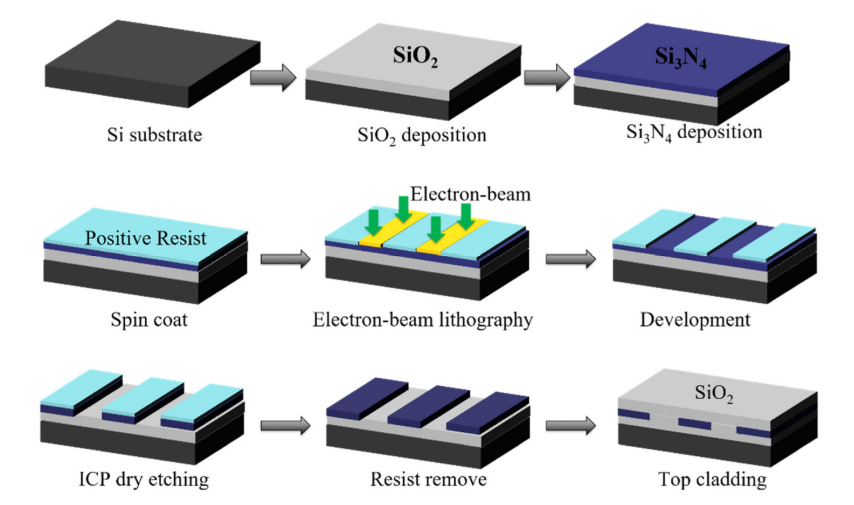
\includegraphics[width=1.0\linewidth]{imgs/png/fab-flow}
	\mycaption{Schematic process flow of the subtractive process}{}
	\label{fig:fab-flow}
\end{figure}

The schematic process flow of the subtractive process is shown in \autoref{fig:fab-flow}. First, the silicon dioxide film is deposited on a 4-inch silicon substrate using the TEOS  (tetraethyl orthosilicate) source.
An alternative method is using a thermal oxidized silicon wafer directly. The target thickness of silicon dioxide layter is greater than 2 \si{\um} to create enough buffer between the silicon nitride film and the silicon substrate. 
Next is silicon nitride film deposition using chemical vapor deposition methods. Following electron beam (EB) lithography patternning, the silicon nitride layer is etched with inductively coupled plasma reactive-ion etching (ICP RIE) technique. After the resist removal, another layer of silica is cladded. Finally, the chip is cut to couple the light from the edge. 

The details of each step will be expanded in the following contents.

%Recently, Si3N4 has been widely utilized in integrated optic devices because of its conspicuous flexibility in the refractive index around 2.0. In our fabrication (Fig. 1), the Si3N4 films with controlled thickness and refractive index were deposited onto the SiO2/Si substrate through LSCVD using the liquid SiN-X source (SAMCO Inc.) with N2 or N2O. The measured refractive index of the deposited Si3N4 film was 1.99, which can be turned to between 1.66 and 1.78 as silicon oxynitride (SiOxNy) by mixing N2O gas. The propagation loss of the films also demonstrated a temperature dependence of the deposition. If the temperature is set too low, the chemical reaction may be uncompleted to form Si3N4. We found that the optimal deposition temperature was 150C to obtain the required low loss properties. The photonic patterns of waveguides, ring resonators, and grating couplers were transferred onto the resist layer on Si3N4 by using the electron beam lithography (EBL) technique. The direct write capability of EBL guarantees the small feature size and high accuracy of the device. After development, the patterned resist was hard-baked at 150C for 5 minutes. This process is effective to improve the dry etching selectivity of the resist and Si3N4, and to help to achieve rectangle waveguide cross-sections. We used a mixed gas of CHF3/O2 for the inductively coupled plasma reactive ion etching (ICP-RIE). After etching to reach the desired depths, we striped the leftover resist using the RIE in which the O2 plasma removes only the resist, but leaves the exposed Si3N4 waveguide untouched. By utilizing CVD, we deposited a top cladding of SiO2 onto the Si3N4 core to form a buried ridge waveguide resonator

\subsection{Film deposition}

Low pressure CVD (LP-CVD) is a traditional method to deposit silicon nitride from the vapor source by the decomposition of chemicals on the surface.  
Stoichiometric silicon nitride can be obtained by controlling and optimizing the ratio of silicon and nitrogen sources. 
The precursor of silicon is usually silane (\ce{SiH4}) or chloride silane gases, such as dichlorosilane (DCS, \ce{SiH2Cl2}). And the ammonia gas (\ce{NH3}) plays the role of nitrogen source. 
\begin{align*}
    \ce{3SiH4(g) + 4NH3(g) &-> Si3N4(s) + 12H2(g)} \\
    \ce{3SiH2Cl2(g) + 4NH3(g) &-> Si3N4(s) + 6HCl(g) + 6H2(g)}
\end{align*}

Considering the toxic gases used in LP-CVD, an alternative approach is to use modern plasma-enhanced CVD (PE-CVD) with liquid source, which has faster growing rate and lower reaction temperature. 

% Although the silicon nitride waveguides deposited by LP-CVD method are mainly reported, it is necessary to figure out the CVD method dependence of film properties, especially the refractive index. 

To compare the CVD method dependence of film properties, especially the refractive index, in our research, three different CVD facilities---LP-CVD, PE-CVD and liquid source CVD (LS-CVD) are exploited with three different recipes to deposit the silicon nitride films.

Compared with commercial silicon nitride on insulator wafers deposited using LP-CVD,
the details of PE-CVD and LS-CVD recipes are listed in \autoref{tab:cvd}. It is apparent from the data that LS-CVD has the fastest rate 23 nm/min, and lowest reaction temperature. In addition, during our experiments, although the flow rate of SN-2 source changes the film growing rate, it does not effect the film stoichiometry and optical properties. 
% This is different from PE-CVD facility used in this research, which can be also used to produce silicon-rich or nitrogen-rich films as controlling the gas ratio.
It is also worth to mention that all the wafer deposited with above three recipes shows no cracks during the fabrication, suggesting low tensile in silicon nitride films.

\begin{table}[]
\centering
\begin{tabular}{cccc}
%\hline
              & LP-CVD                            & PE-CVD                                                                                  & LS-CVD                                                                                  \\ \hline
Facility      & -                                 & SAMCO PD-220NL                                                                          & SMACO PD-100ST                                                                          \\ \hline
Source        & DCS:NH3:N2                        & \begin{tabular}[c]{@{}c@{}}\ce{SiH4}:\ce{NH3}:N2\\ =6:5:189 sccm\end{tabular}                     & \begin{tabular}[c]{@{}c@{}}SN-2:\ce{N2}\\ =0.5:30 sccm\end{tabular}                          \\ \hline
Chamber Temp. & 750\si{\celsius}-800\si{\celsius} & \begin{tabular}[c]{@{}c@{}}upper 150\si{\celsius}\\ lower 350\si{\celsius}\end{tabular} & \begin{tabular}[c]{@{}c@{}}upper 150\si{\celsius}\\ lower 180\si{\celsius}\end{tabular} \\ \hline
RF Power      & -                                 & 40 W                                                                                     & 30 W                                                                                     \\ \hline
Deposition Rate          & -                                 & 15 nm/min                                                                               & 23 nm/min                                                                               \\ \hline
\end{tabular}
\mycaption{Recipes of CVD methods used in this research}{In the case of PE-CVD and LS-CVD, upper electrode and lower electrode are set at different temperature. RF power refers to radio frequency power used to excite the precursor gasses.}
\label{tab:cvd}
\end{table}


\subsection{Material properties}

\subsubsection{Ellipsometry}

It is more necessary to evaluated the refractive indexes of the film deposited above. Using the infrared elliposometry, the refractive index of deposited silicon nitride film is obtained. The result is shown in \autoref{fig:ellipso}, where we can see the index varies from the deposition methods at the magnitude of 0.01.
Furthermore, even the refractive index are distinguished, the material wavelength dispersion parameter $D_M$ can be close.

\subsubsection{Fourier-transform infrared spectroscopy}

The vast majority of studies on silicon nitride fabrication processes have found that the hydrogen remaining in the films leads to N-H and Si-H bonds, which causes the optical absorption at S and C band \cites{Ay2004, Agnihotri2000}. To quantitatively clarify these bonds in our film, we perform the Fourier-transform infrared spectroscopy (FTIR) on the top of silicon nitride film.

The measurement is carried out using attenuated total reflection (ATR) method with SHIMADZU ?. In \autoref{fig:ftir}, the absorbance is taken from the difference with background transmittance. It can be seen that except the peak around 800? \si{\per\cm} referring to Si-N stretching mode, two other peaks are located around 2150 and 3350 \si{\per\cm}, corresponding to Si-H and N-H bonds respectively.

Interestingly, there are also two peaks found at 1020 and 1120, indicating Si-O symmetric and asymmetric stretching modes. This result may be explained by the fact that in ATR method, the depth of penetration at this wavelength is less than 1 micron, while the thickness of silicon nitride layers in our experiment is targeted at 800 nm.
% \cite{Shaw2005}


\begin{figure}
    \centering
    \includesvg[width=.6\textwidth]{ftir}
    \caption{Caption}
    \label{fig:ftir}
\end{figure}

In conclusion, even though the ammonia free recipe is used in LS-CVD method, the film is still hydrogenated while LP-CVD commercial wafers show least N-H absorbance.



\begin{figure}
	\centering
	\includesvg[scale=0.8]{ellipso}
	\mycaption{Elliposometry result of the film deposited in several method}{}
	\label{fig:ellipso}
\end{figure}



\subsection{Patterning}
The sample used in our experiments are usually in the size of 20 mm $\times$ 20 mm, diced off from a 4-inch wafer. Before the electron beam lithography, electron beam resist is spin-coated on the surface of silicon nitride films after several times of cleaning. 

But first, a layer of an adhesion promoter, hexamethyldisilazane (HDMS) is coated at 2000 rpm and then baked at 120 \si{\celsius} for 1 min. Next, the positive resist (AR-P 6500, ALLRESIST GmbH) is coated at 1000 rpm and soft-baked at 120 \si{\celsius} for 2 min. The final thickness of resist is around 800 nm to achieve enough thickness during the etching process. The main EB machine used in our experiments is ELIONIX ELS-F100 and the beam dose is 3 nA, 0.6 sec/dot. This recipe is fully optimized and has small feature sizes and high accuracy around 10 nm. After the lithography, the sample is developed using \textit{o}-xylene. 

% Several EB resists are compared, both negative and positive type. 

\subsection{ICP etching}

In order to etch the waveguide layer selectively, ICP-RIE (RIE-400iPB, SAMCO Inc.) is used to remove the unmasked section in silicon nitride layer.

Different from previous work \cite{Yusuke2017}, the ICP-RIE facility used in this study is optimized for deep silicon etching. In the key etching step of our recipe, only \ce{CHF3} gas, 6 sccm, is used along with argon gas to cleans any residual organic matter over the surface. ICP power is set 50 W, and RF bias power is 20 W.

The etching rate of three kinds of film is listed in \autoref{tab:cvd}. From the data, we can see LS-CVD deposited film has the best selectivity, much higher than LP- and PE-CVD samples. It seems possible that the film density varies from the CVD methods, due to LS-CVD has the fastest growth rate and lowest reaction temperature.

\begin{table}[]
\begin{tabular}{cccc}
%\hline
       & \begin{tabular}[c]{@{}c@{}}Film Etching Rate \\ (nm/min)\end{tabular} & \begin{tabular}[c]{@{}c@{}}Resist Etching Rate\\ (nm/min)\end{tabular} & Selectivity \\ \hline
LP-CVD & 19.20                                                            & 12.76                                                                     & 1.50        \\ \hline
PE-CVD & 23.48                                                            & 14.29                                                                     & 1.64        \\ \hline
LS-CVD & 27.40                                                            & 2.08                                                                      & 13.17       \\ \hline
\end{tabular}
\mycaption{Etching rate and selectivity of ICP process}{}
\label{tab:icp}
\end{table}

\subsection{Top-cladding and annealing}
The final step is cladding another layer of silicon dioxide. 
%Several works refer that low-temperature oxide can be lossy b
To remove not only the residual EB resists but also the polymer generated during the plasma etching, 
all the samples are first deeply ashed using normal oxygen recipe in another RIE facility. To reduce the damage to the waveguide shape during ashing, organic cleaning is supplied. As same as the buried oxide layer, TEOS source is used to deposit a 2-3 \si{\um} top cladding layer with the same LS-CVD facility.

% \citeauthor{Ang2018} founds 
To remove the residual hydrogen in silicon nitride film, an optional step of annealing is necessary. 

Traditionally, annealing process can be performed in different cases, after or during CVD deposition \cite{Luke2013}, after dry etching or after top cladding \cite{Ang2018}. Since the first case requires tensile control during cycled deposition-annealing operation \cite{Luke2013}, in our experiments, annealing before or after top cladding of negatively patterned LS-CVD and PE-CVD sample are merely compared.

To achieve high vacuum during the annealing, we use a tube-type electric furnace. In a high vacuum, the furnace is set first heating gradually  from room temperature to 300 \si{\celsius} for 1 h, then heating to 1000 \si{\celsius} for 3 h, keeping at 1000 \si{\celsius} for 4 h, and cooling down to 300 \si{\celsius} for 5 h, then naturally cooling to room temperature. 

Shown in \autoref{fig:anneal}, there are cracks on both the LS-CVD and PE-CVD samples. In contrast, the negatively patternned samples are free of any cracks but is severely contaminated, which possibly results from the contamination in the tube furnace. 
In general, the finding of cracks on the top clad layer shows despite the tensile control over the silicon nitride film, even negative EB resist is used for transferring the structure, it is still difficult to annealing the typical TEOS cladded samples with the PE-CVD facility in our fabrication condition.

\begin{figure}
    \centering
    \begin{subfigure}[b]{0.45\textwidth}
    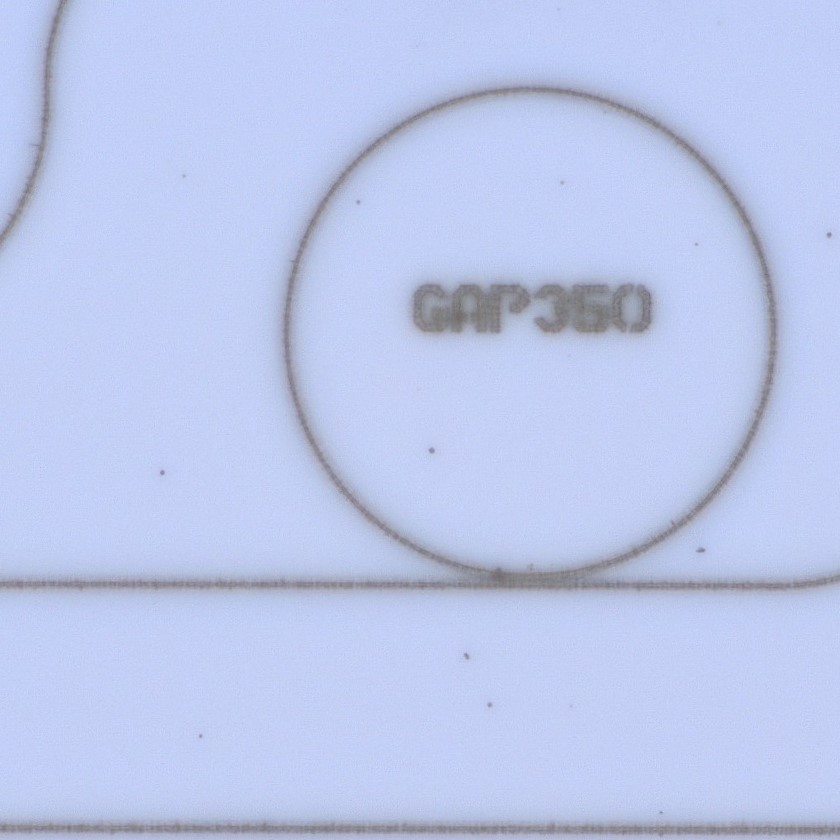
\includegraphics[width=\textwidth]{imgs/jpg/LS_ac}
    \caption{}
    \end{subfigure}
    \begin{subfigure}[b]{0.45\textwidth}
    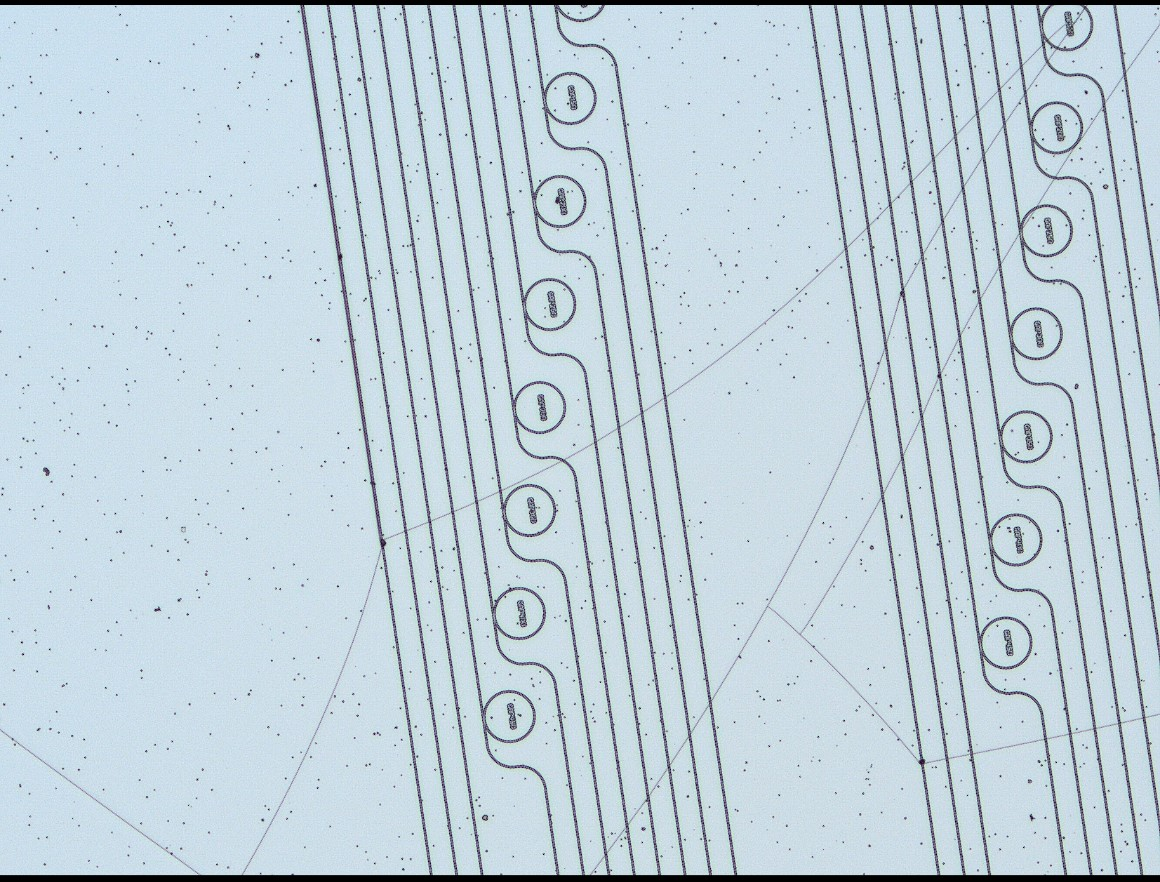
\includegraphics[width=\textwidth]{imgs/jpg/LS_tc}
    \caption{}
    \end{subfigure}    
    \begin{subfigure}[b]{0.45\textwidth}
    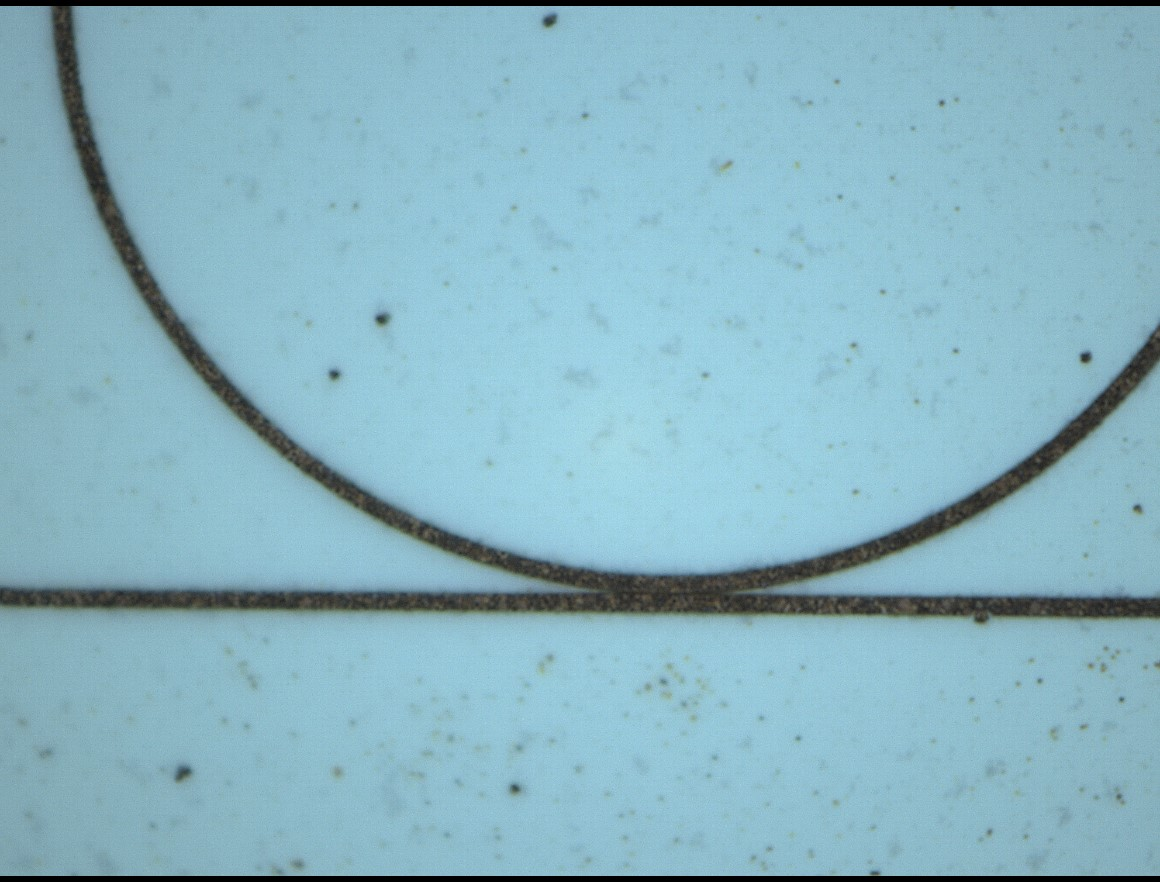
\includegraphics[width=\textwidth]{imgs/jpg/SR_ac}
    \caption{}
    \end{subfigure}
    \begin{subfigure}[b]{0.45\textwidth}
    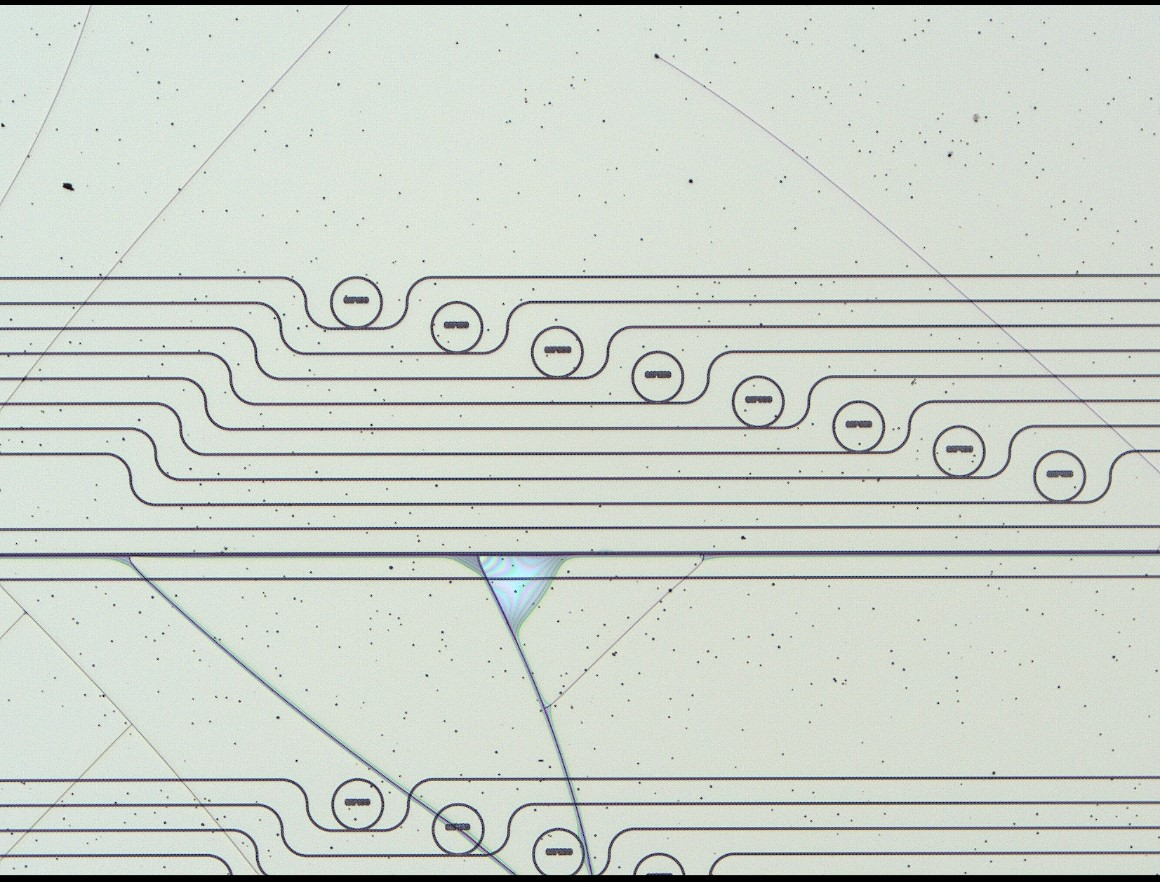
\includegraphics[width=\textwidth]{imgs/jpg/SR_tc}
    \caption{}
    \end{subfigure}
    \mycaption{Laser microscope images of samples after annealing process}{All the sample are annealed under the same circumstance. \textbf{a}. LS-CVD sample without top cladding. \textbf{b}. LS-CVD sample with TEOS top-cladding. \textbf{c}. PE-CVD sampele without top cladding. \textbf{d}. PE-CVD sample with TEOS top-cladding.}
    \label{fig:anneal}
\end{figure}

\subsection{Edge coupling and chip dicing}\label{sec:chip-dicing}

To achieve high coupling efficiency, we adopt monolithic inversed tapered waveguide as the mode convertor. The input and output ports of waveguide are both tapered from normal width 1.5 \si{\um} to a narrower end. By FDTD methods, the mode field is swept with different taper end widths.

\begin{figure}
	\centering
	\begin{subfigure}[b]{0.33\textwidth}
		\includesvg[width=\textwidth]{taper/03.svg}
		\caption{End width 0.3 \si{\um}}
	\end{subfigure}\hfill
	\begin{subfigure}[b]{0.33\textwidth}
		\includesvg[width=\textwidth]{taper/06}
		\caption{End width 0.6 \si{\um}}
	\end{subfigure}\hfill
	\begin{subfigure}[b]{0.33\textwidth}
		\includesvg[width=\textwidth]{taper/09}
		\caption{End width 0.9 \si{\um}}
	\end{subfigure}
	\vfill
	\begin{subfigure}[b]{0.33\textwidth}
		\includesvg[width=\textwidth]{taper/12}
		\caption{End width 1.2 \si{\um}}
	\end{subfigure}
	\begin{subfigure}[b]{0.33\textwidth}
		\includesvg[width=\textwidth]{taper/15}
		\caption{End width 1.5 \si{\um}}
	\end{subfigure}
    \mycaption{Mode field at the taper end}{The outline of taper edge is profiled.}
\label{fig:taper}
\end{figure}

From the result shown in \autoref{fig:taper}a, the mode fields expand horizontally as the taper end width increases proportionally. The largest mode size of 3.4 \si{\um} $\times$ 3.4 \si{\um} is successfully demonstrated, but the enhancement is not significant compared with no tapered port in \autoref{fig:taper}e. In result, a lensed fiber with spot diameter from 3.0 \si{\um} to 3.4 \si{\um} is recommended. 

In order to precisely define the input and output ports, the chip dicing is required.
Compared with conventional mechanical dicing,  the laser dicing technique is advantageous at high precision and less damages on the chip edges. The image of laser diced edge is compared with the manually diced one in \autoref{fig:dicing}. Apparently, the chip using laser dicing has smoother edge, which is helpful to reduce the backward scattering.

\begin{figure}
    \centering
	\begin{subfigure}[b]{0.45\textwidth}
		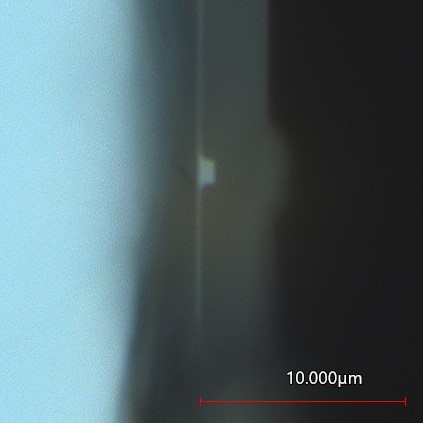
\includegraphics[width=\textwidth]{imgs/jpg/laser}
 		\caption{Laser diced}
	\end{subfigure}
	\begin{subfigure}[b]{0.45\textwidth}
		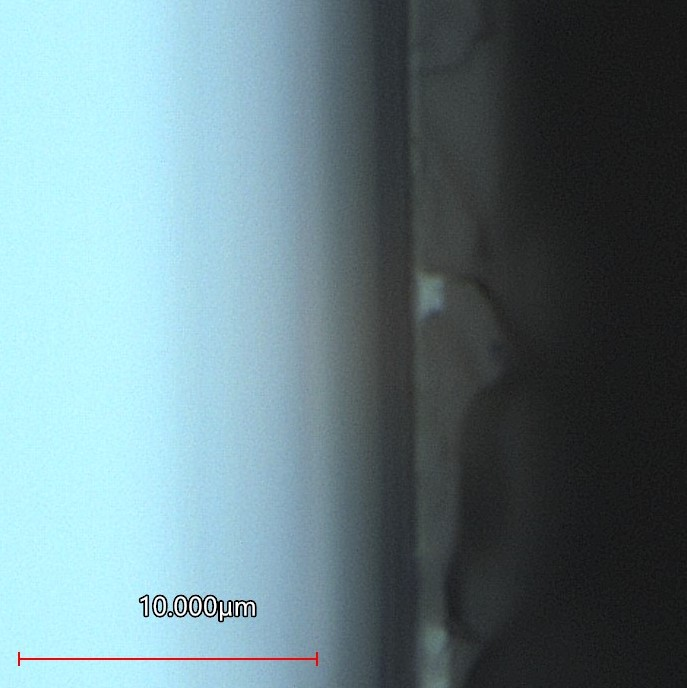
\includegraphics[width=\textwidth]{imgs/jpg/manual_cleav}
 		\caption{Manually cleaved}
	\end{subfigure}
    \mycaption{Microscope images of chip edge}{The scale in the images is 10 \si{um}.}
    \label{fig:dicing}
\end{figure}

\section{Fabless samples via foundries}

Fabless photonic research is becoming a trend for its cheaper and easier external run \cite{Hochberg2010}. There are several foundries all around the world offering the multi-project run service on integrated photonics and quantum optics applications, such as AMF in Singapore, Ligentec in Switterland, LioniX in Netherlands and etc. 

Based on the silicon nitride platform, two independent foundries are evaluated in the following sections in the term of device performance and fabrication techniques.

\subsection{Ligentec technique}
Photonic damascene process \cite{Pfeiffer2015a,Pfeiffer2018a} used in Ligentec samples improves the waveguide sidewall roughness by depositing the silicon nitride film into the etched thermal oxidized silica. By additive chemical mechanical planarization (CMP), the top surface of silicon nitride is improved.

The sample layout is illustrated in \autoref{fig:gds_ligentec}. Five groups of various FSRs are designed. In ecch specific group, the coupling gap is detuned gradually from 400 nm to 700 nm in the step of 100 nm.


\begin{table}[]
\begin{tabular}{cccc}
% \hline
        & Ring Radius (\si{\um}) & FSR (GHz) & Ring Width (\si{\um}) \\ \hline
Group 1 & 200                                                    & 100       & 0.8                                                   \\ \hline
Group 2 & 200                                                    & 150       & 1.7                                                   \\ \hline
Group 3 & 200                                                    & 200       & 1.5                                                   \\ \hline
Group 4 & 10                                                     & 300       & 1.7                                                   \\ \hline
Group 5 & 30                                                     & 1000      & 1.7                                                   \\ \hline
\end{tabular}
\end{table}

The microscope images of the samples is shown in \autoref{fig:ligentec-laser-micro}. Several layers of different structures are observed hierarchically, including the cross pattern stopping the crack during annealing and CMP, the silicon waveguides and a top unknown metallic layer.

\begin{figure}
    \centering
    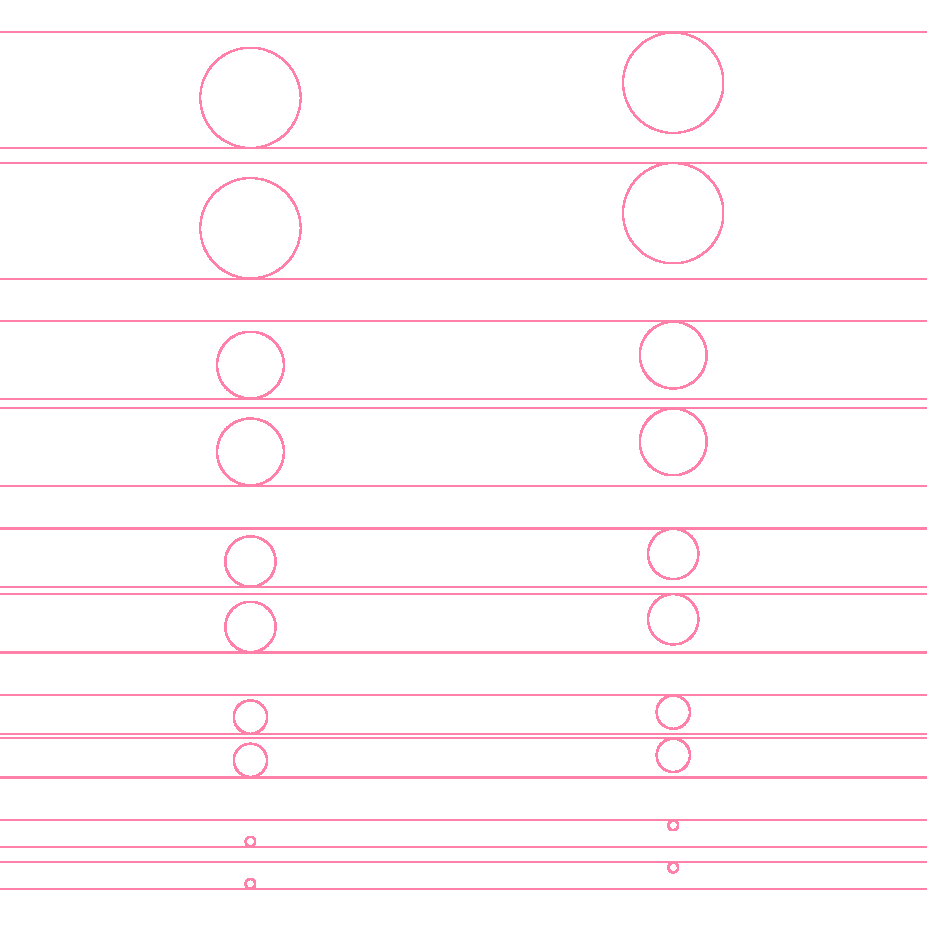
\includegraphics[width=.6\textwidth]{imgs/png/ligentec_gds}
    \caption{Caption}
    \label{fig:gds_ligentec}
\end{figure}

\begin{figure}
	\centering
	\begin{subfigure}[b]{0.45\textwidth}
		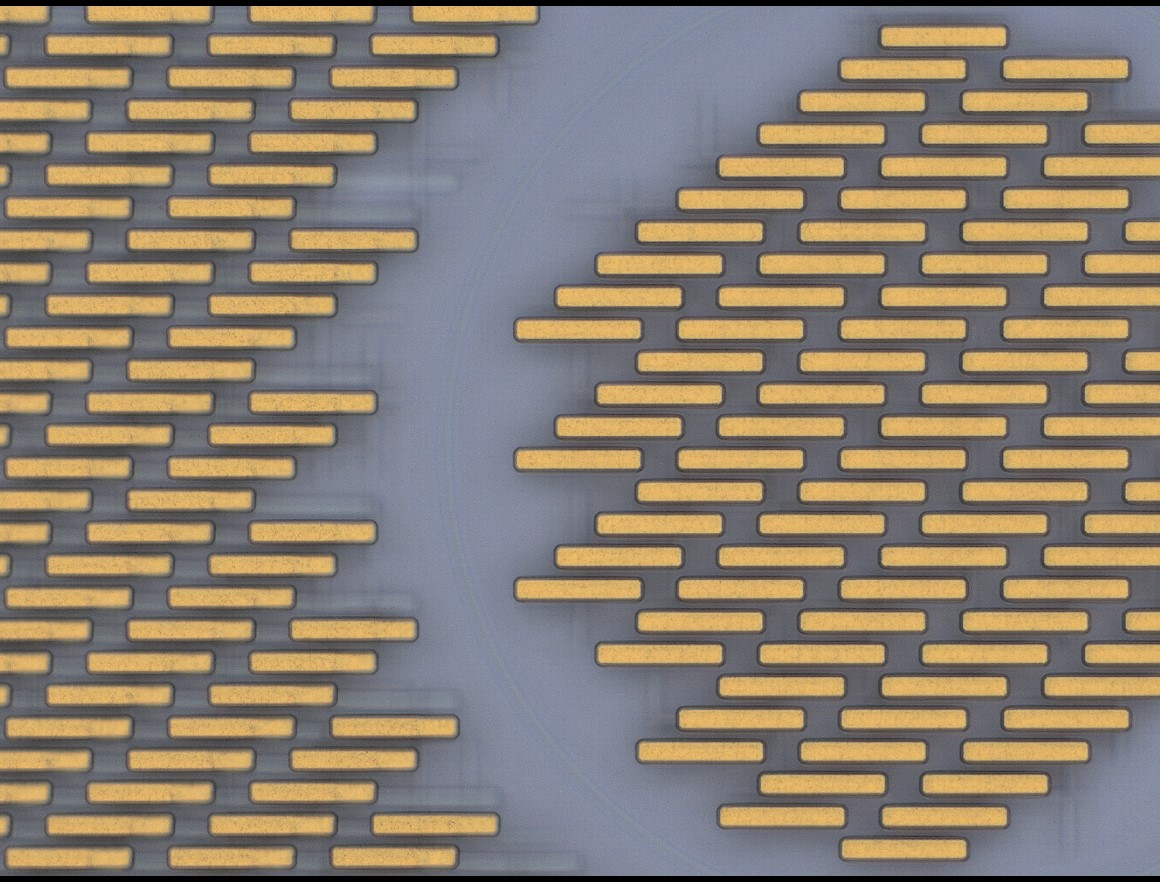
\includegraphics[width=\textwidth]{imgs/jpg/ligentec/top}
		\caption{}
	\end{subfigure}
	\begin{subfigure}[b]{0.45\textwidth}
		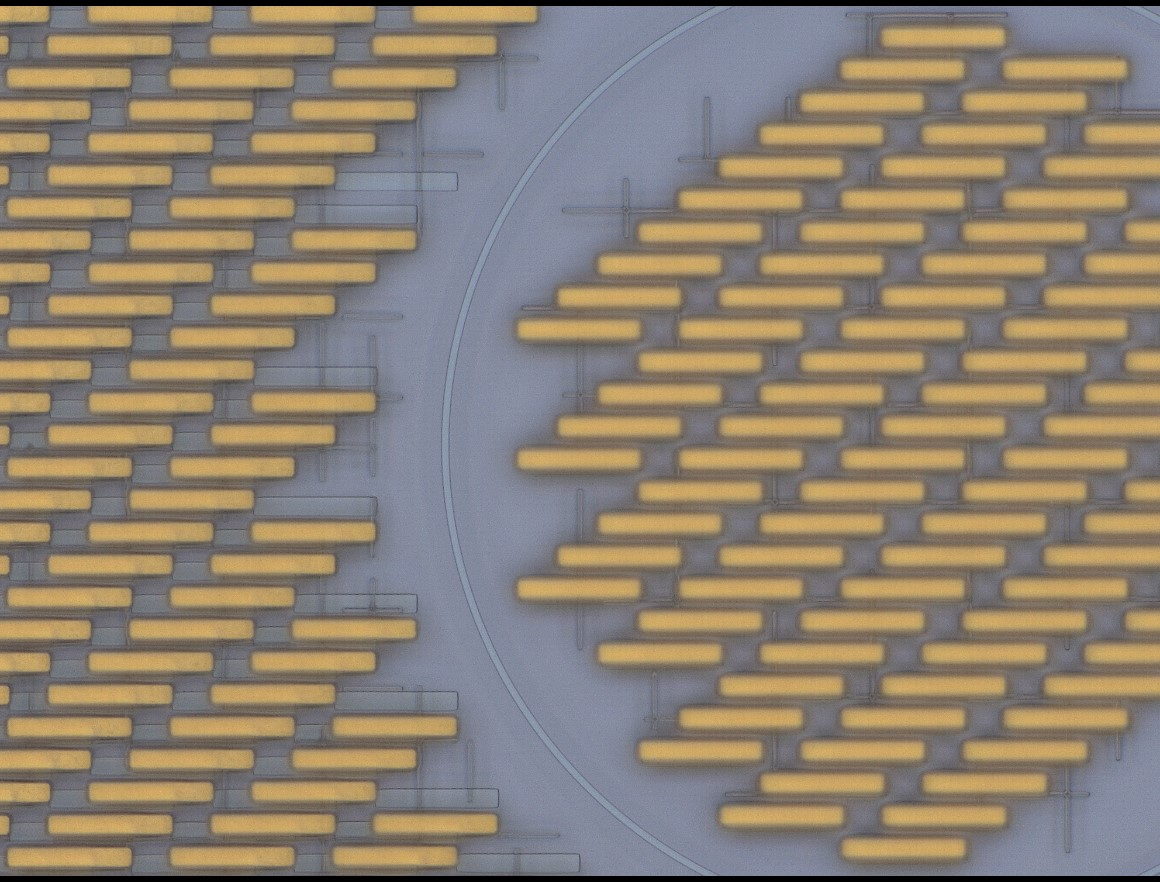
\includegraphics[width=\textwidth]{imgs/jpg/ligentec/dev}
		\caption{}
	\end{subfigure}
	\begin{subfigure}[b]{0.45\textwidth}
		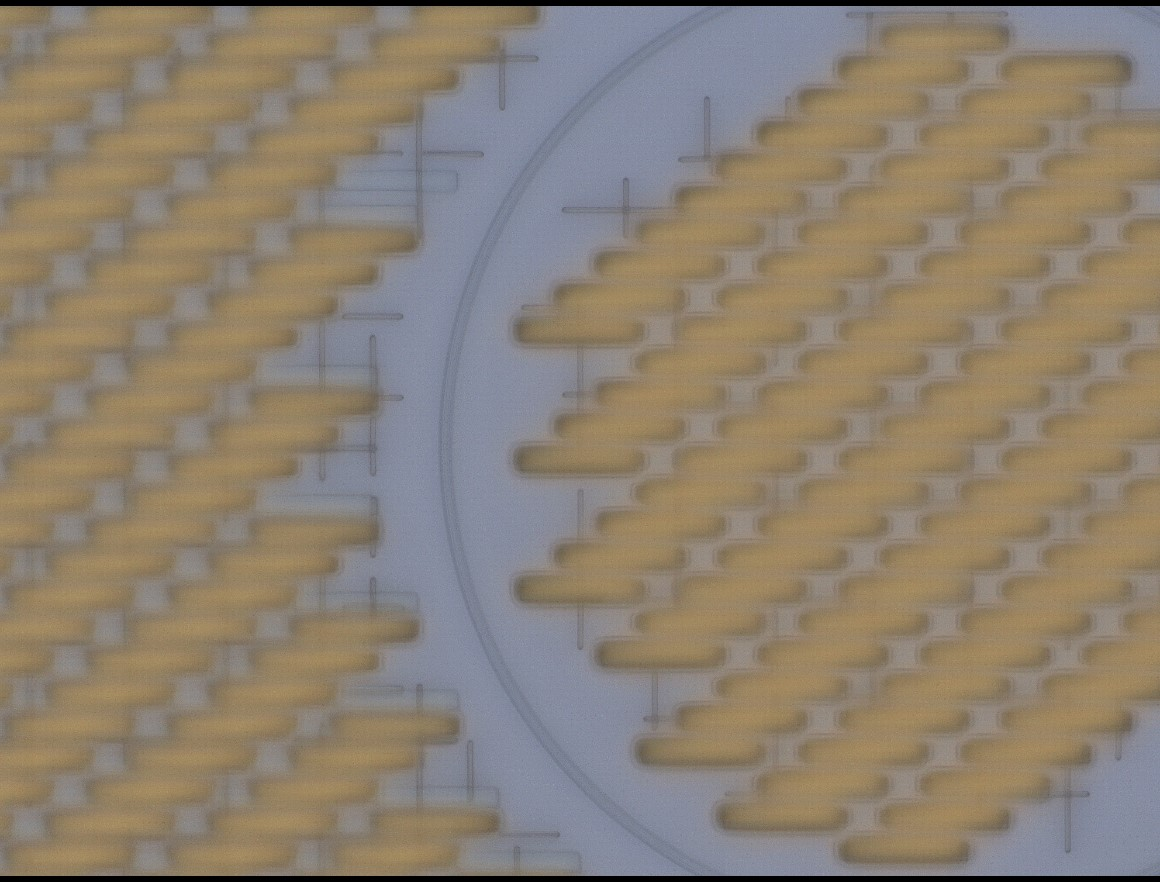
\includegraphics[width=\textwidth]{imgs/jpg/ligentec/cross}
		\caption{Crack stopper layer}
	\end{subfigure}
	\begin{subfigure}[b]{0.45\textwidth}
		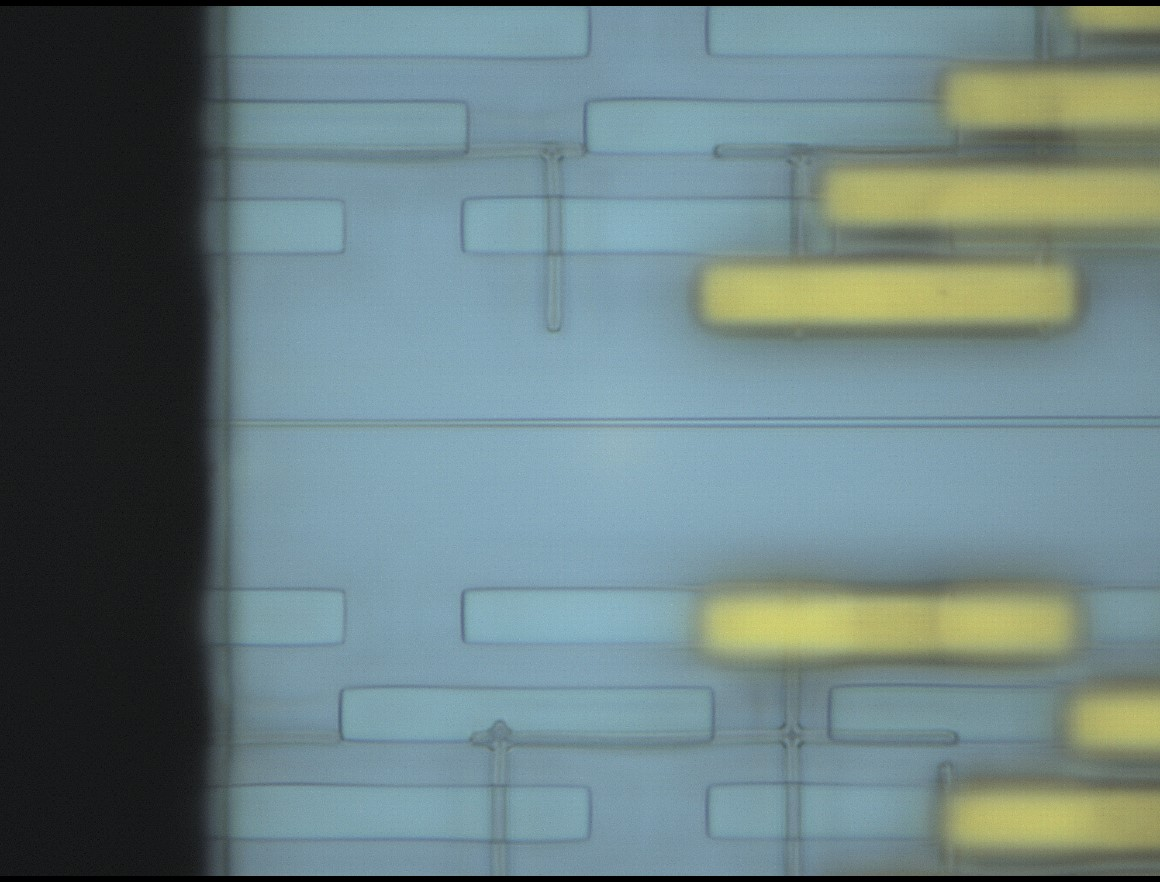
\includegraphics[width=\textwidth]{imgs/jpg/ligentec/cov}
		\caption{}
	\end{subfigure}
	\mycaption{Laser microscope images of Ligentec smaples}{By lowering the focus depth, three layers are observed.
	\textbf{a}. Top metallic layer. \textbf{b}. Device layer. \textbf{c}. Crack stopper layer. \textbf{d}. Mode convertor}
	\label{fig:ligentec-laser-micro}
\end{figure}

\subsection{NTT-AT technique}


NTT-AT technique adopts a different physical vapor method--reactive sputtering to deposit non-hydrogen silicon nitride. Compared with standard silicon sputtering, the nitrogen flow is supplied and reacts with silicon vapor into the silicon nitride film. The refractive index of the film deposited using method is also shown in \autoref{fig:ellipso}.

\begin{figure}
    \centering
    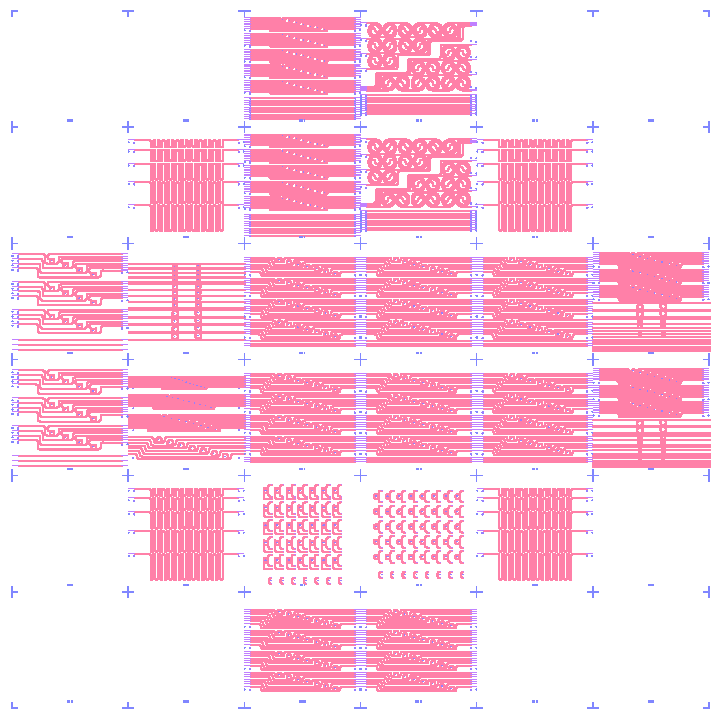
\includegraphics[width=\textwidth]{imgs/png/ntt_gds.png}
    \caption{Caption}
    \label{fig:gds_ntt}
\end{figure}

% Despite the hydrogen bond induced loss.